\section{XMCascade\-Button  Class Reference}
\label{classXMCascadeButton}\index{XMCascadeButton@{XMCascade\-Button}}
{\tt \#include $<$XMPushbutton.h$>$}

Inheritance diagram for XMCascade\-Button::\begin{figure}[H]
\begin{center}
\leavevmode
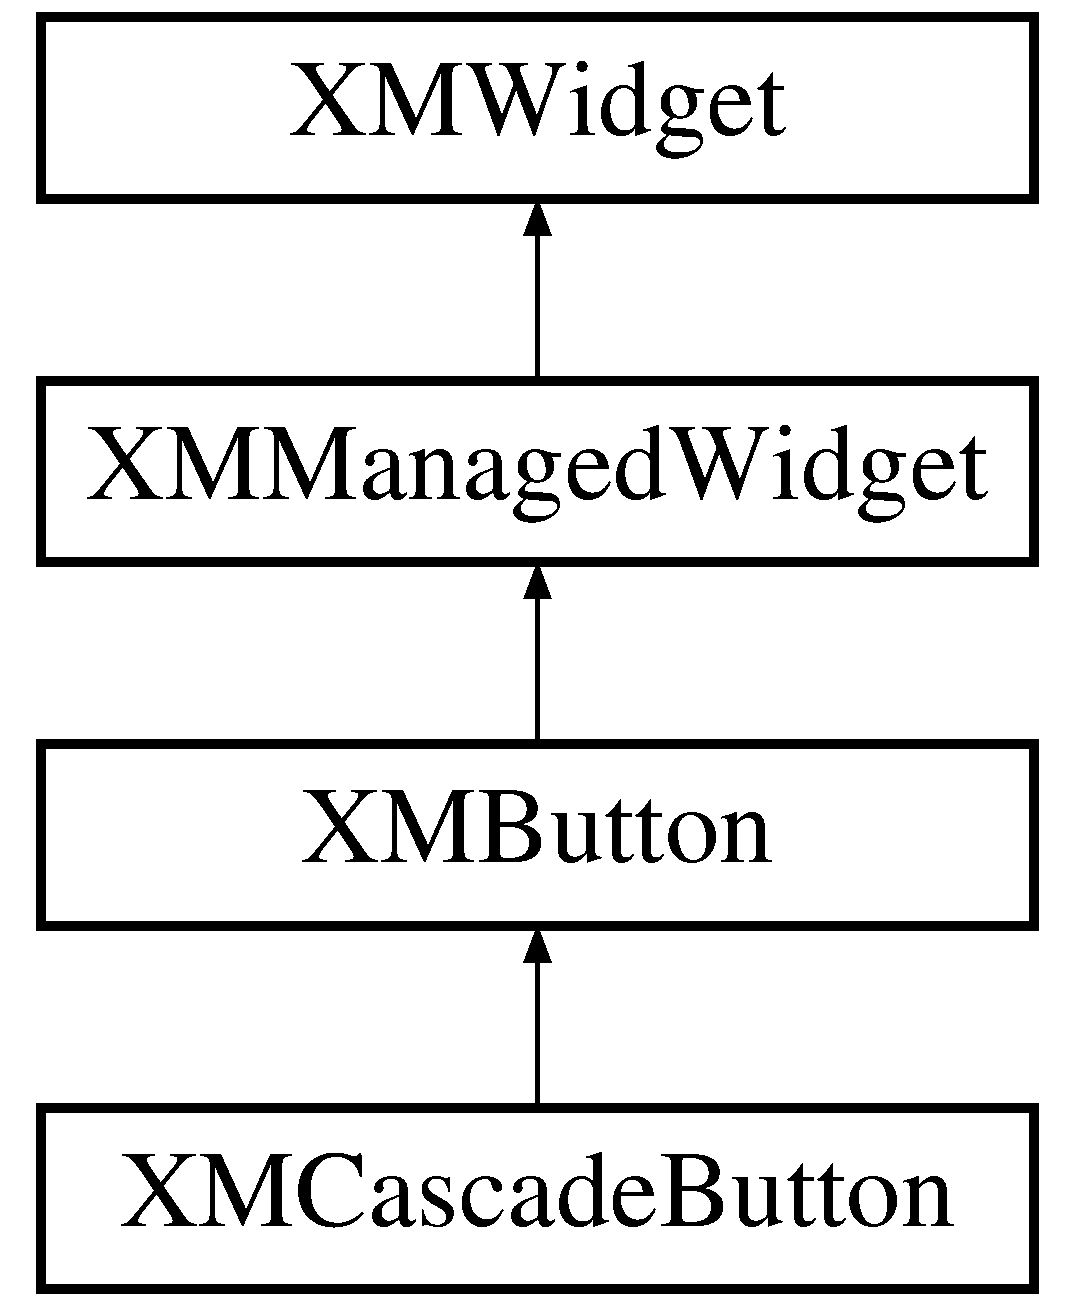
\includegraphics[height=4cm]{classXMCascadeButton}
\end{center}
\end{figure}
\subsection*{Public Methods}
\begin{CompactItemize}
\item 
void {\bf Set\-Associated\-Menu} ({\bf XMWidget} \&w)
\item 
void {\bf Set\-Associated\-Menu} (Widget w)
\item 
{\bf XMCascade\-Button} (char $\ast$n, Widget parent, void($\ast$cb)({\bf XMWidget} $\ast$, Xt\-Pointer, Xt\-Pointer)=NULL, Xt\-Pointer cd=NULL)
\item 
{\bf XMCascade\-Button} (char $\ast$n, {\bf XMWidget} \&parent, void($\ast$cb)({\bf XMWidget} $\ast$, Xt\-Pointer, Xt\-Pointer)=NULL, Xt\-Pointer cd=NULL)
\item 
{\bf XMCascade\-Button} (Widget w)
\item 
{\bf Callback\_\-data} $\ast$ {\bf Add\-Callback} (void($\ast$cb)({\bf XMWidget} $\ast$, Xt\-Pointer, Xt\-Pointer)=NULL, Xt\-Pointer cd=NULL)
\end{CompactItemize}


\subsection{Constructor \& Destructor Documentation}
\index{XMCascadeButton@{XMCascade\-Button}!XMCascadeButton@{XMCascadeButton}}
\index{XMCascadeButton@{XMCascadeButton}!XMCascadeButton@{XMCascade\-Button}}
\subsubsection{\setlength{\rightskip}{0pt plus 5cm}XMCascade\-Button::XMCascade\-Button (char $\ast$ {\em n}, Widget {\em parent}, void($\ast$ {\em cb})({\bf XMWidget} $\ast$, Xt\-Pointer, Xt\-Pointer) = NULL, Xt\-Pointer {\em cd} = NULL)\hspace{0.3cm}{\tt  [inline]}}\label{classXMCascadeButton_a2}




Definition at line 431 of file XMPushbutton.h.

References XMWidget::Add\-Callback(), and XMButton::Enable().\index{XMCascadeButton@{XMCascade\-Button}!XMCascadeButton@{XMCascadeButton}}
\index{XMCascadeButton@{XMCascadeButton}!XMCascadeButton@{XMCascade\-Button}}
\subsubsection{\setlength{\rightskip}{0pt plus 5cm}XMCascade\-Button::XMCascade\-Button (char $\ast$ {\em n}, {\bf XMWidget} \& {\em parent}, void($\ast$ {\em cb})({\bf XMWidget} $\ast$, Xt\-Pointer, Xt\-Pointer) = NULL, Xt\-Pointer {\em cd} = NULL)\hspace{0.3cm}{\tt  [inline]}}\label{classXMCascadeButton_a3}




Definition at line 441 of file XMPushbutton.h.

References XMWidget::Add\-Callback(), and XMButton::Enable().\index{XMCascadeButton@{XMCascade\-Button}!XMCascadeButton@{XMCascadeButton}}
\index{XMCascadeButton@{XMCascadeButton}!XMCascadeButton@{XMCascade\-Button}}
\subsubsection{\setlength{\rightskip}{0pt plus 5cm}XMCascade\-Button::XMCascade\-Button (Widget {\em w})\hspace{0.3cm}{\tt  [inline]}}\label{classXMCascadeButton_a4}




Definition at line 451 of file XMPushbutton.h.

\subsection{Member Function Documentation}
\index{XMCascadeButton@{XMCascade\-Button}!AddCallback@{AddCallback}}
\index{AddCallback@{AddCallback}!XMCascadeButton@{XMCascade\-Button}}
\subsubsection{\setlength{\rightskip}{0pt plus 5cm}{\bf Callback\_\-data}$\ast$ XMCascade\-Button::Add\-Callback (void($\ast$ {\em cb})({\bf XMWidget} $\ast$, Xt\-Pointer, Xt\-Pointer) = NULL, Xt\-Pointer {\em cd} = NULL)\hspace{0.3cm}{\tt  [inline]}}\label{classXMCascadeButton_a5}




Definition at line 455 of file XMPushbutton.h.

References XMWidget::Add\-Callback().\index{XMCascadeButton@{XMCascade\-Button}!SetAssociatedMenu@{SetAssociatedMenu}}
\index{SetAssociatedMenu@{SetAssociatedMenu}!XMCascadeButton@{XMCascade\-Button}}
\subsubsection{\setlength{\rightskip}{0pt plus 5cm}void XMCascade\-Button::Set\-Associated\-Menu (Widget {\em w})\hspace{0.3cm}{\tt  [inline]}}\label{classXMCascadeButton_a1}




Definition at line 421 of file XMPushbutton.h.

References XMWidget::Set\-Attribute().\index{XMCascadeButton@{XMCascade\-Button}!SetAssociatedMenu@{SetAssociatedMenu}}
\index{SetAssociatedMenu@{SetAssociatedMenu}!XMCascadeButton@{XMCascade\-Button}}
\subsubsection{\setlength{\rightskip}{0pt plus 5cm}void XMCascade\-Button::Set\-Associated\-Menu ({\bf XMWidget} \& {\em w})\hspace{0.3cm}{\tt  [inline]}}\label{classXMCascadeButton_a0}




Definition at line 417 of file XMPushbutton.h.

References XMWidget::getid(), and XMWidget::Set\-Attribute().

Referenced by XMPulldown::Build\-Menu().

The documentation for this class was generated from the following file:\begin{CompactItemize}
\item 
{\bf XMPushbutton.h}\end{CompactItemize}
